% Status: Erstkorrektur
% Designdarstellung.tex

\subsection{Designpräsentation}
Die Designpräsentation basiert ebenfalls auf dem SVG-Format, welche durch die React-Komponente \lstinline|DesignPresenter.tsx| erzeugt wird. 

Die Abbildung \ref{fig:Designdarstellung} weißt die Abhängigkeiten der Designpräsentation auf.

\begin{figure}[H]
    \centering
    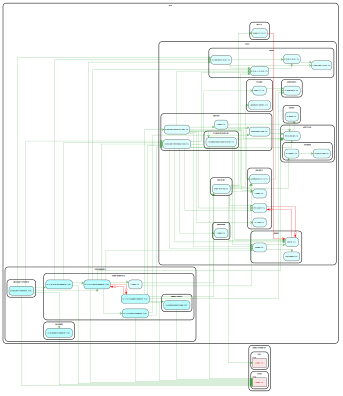
\includegraphics[width=1\textwidth]{diagrams/Ist-Architektur/design-presenter-analysis.pdf}
    \caption{Abhängigkeiten der Komponenten für Designdarstellung}
    \label{fig:Designdarstellung}
\end{figure}

Die React-Komponente \lstinline|DesignPresenter.tsx| erzeugt, basierend auf eine Designstruktur welche innerhalb der Datei \lstinline|src/core/entities/FDDesign.ts| definiert ist, die SVG-Struktur zur Darstellung im Browser. Die Datei \lstinline|FDDesign.ts| enthält eine Sammlung von Schnittstellen, welche die verschieden Elemente eine Designs beschreiben.   
Ein Darstellung der Strukturierung der Schnittstellen als Klassediagramm ist im Anhang unter \emph{D1\_FDDesign.pdf} enthalten.

Die Designpräsentation wird der Produktpräsentation als Kindkomponente übergeben. Dadurch sind beiden React-Komponenten voneinander entkoppelt und das Design wird lediglich innerhalb der Produktdarstellung dargestellt.

Folgende Bausteine wurden aus den Abhängigkeiten der Designpräsentation extrahiert.
\begin{multicols}{2}
\begin{enumerate}
\item Bildverarbeitung 
\item Cache 
\item Designdarstellung 
\item Designobjekt-Transformation 
\item Designobjekterzeugung 
\item Designstruktur 
\item Farbstruktur 
\item JavaScript-Erweiterung 
\item Mathematik  
\item Maßeinheit-Konverter 
\item Produktstruktur 
\item Schriftverarbeitung 
\item SVG-Parser 
\item XML-Parser 
\end{enumerate}
\end{multicols}